%% ch06-ai-synthesis.tex — Chapter VI: Learned Synthesis and Honest Cost Accounting
%% Sources: guo2026rubriq, guo2026rubriqsoftware, guo2026nonlinearwaves, guo2026splitstepqude
%% Label prefix: syn:
\chapter{Learned Synthesis and Honest Cost Accounting}\label{ch:synthesis}

\authorshipstatement{This chapter is based on two manuscripts. Part~A follows Z.~Guo and Z.~Pan, ``\rubriq{}: Rubric-Guided Group Relative Policy Optimization for Constraint-Aware Quantum Circuit Synthesis,'' arXiv:2607.07554 (2026), posted on Research Square and under review at \emph{npj Quantum Information}~\cite{guo2026rubriq}; the software artifact is archived on Zenodo~\cite{guo2026rubriqsoftware}. Part~B follows Z.~Guo, V.~Dsouza, A.~Khan, A.~Chopra, R.~Lineswala and Z.~Pan, ``Measurement and Reload Costs in Direct Quantum Simulation of Nonlinear Waves,'' arXiv:2608.21647 (2026)~\cite{guo2026nonlinearwaves}; code and data are archived as SplitStepQUDE~\cite{guo2026splitstepqude}. For \rubriq{} the candidate conceived the rubric-reward formulation, implemented the training and evaluation software, ran all experiments on Perlmutter and on the IBM and IonQ devices, and wrote the manuscript; Z.~Pan supervised the work. For the nonlinear-wave study the candidate designed the hybrid split-step solver, the cost model and the adaptive controller, implemented the quantum kernels, ran the simulations and hardware experiments, and wrote the manuscript; the coauthors from BosonQ Psi contributed the application setting and classical reference solutions and advised on the numerical analysis; Z.~Pan supervised the work.}
% TODO (author action, not printed): confirm this contribution statement with all coauthors before submission.


This chapter addresses RQ4: can learned, HPC-scale synthesis produce circuits that respect fault-tolerant resource budgets, and what does honest cost accounting say about end-to-end quantum advantage? The two halves of the question are answered by two studies that share a method---put the full cost of a quantum computation into a single, programmatic accounting and let that accounting drive the design. Part~A (\crefrange{sec:syn:prelim}{sec:syn:rubriq-discussion}) presents \rubriq{}, which casts fault-tolerant circuit synthesis as large-language-model (LLM) code generation fine-tuned by reinforcement learning against a rubric that scores fidelity, Clifford fraction, topology compliance, T-gate count and efficiency, with GPU-accelerated \cudaq{} simulation inside the training loop. Part~B (\cref{sec:syn:waves}) asks what it costs to simulate nonlinear wave equations on a quantum processor when the nonlinearity needs the field itself, and answers with a unified measurement-and-reload cost model that is validated on hardware. The chapter closes by relating both studies to the rest of the dissertation (\cref{sec:syn:relation}) and summarizing (\cref{sec:syn:summary}).

\section{Introduction}\label{sec:syn:intro}

The previous chapters scaled simulation (\cref{ch:qgear}), made the classical--quantum data interface vectorized and learnable (\cref{ch:qml}) and replaced black-box variational search with problem structure (\cref{ch:nisq}). Each of those contributions was measured against the hardware that exists today. This chapter turns toward the hardware that is being built: fault-tolerant processors whose cost model is dominated not by two-qubit gate error but by the number of non-Clifford operations that must be distilled~\cite{bravyi2005magic,fowler2012surfacecodes}. In that regime a compiler is judged by a different question. It is no longer ``how few CZ gates?'' but ``how few T gates, on the right topology, without breaking the function the circuit is meant to implement?''

Classical circuit synthesis attacks that question with heuristics and search. T-count and T-depth optimizers based on phase-polynomial and matroid techniques~\cite{amy2014tpar} are exact for restricted gate sets but do not scale to structured algorithmic circuits, and exhaustive synthesis is exponential in the number of qubits. Generative models have recently entered the field: diffusion models can propose circuits for small unitaries~\cite{furrutter2024genqc}, and code-generating LLMs~\cite{chen2021codex} can already write \qiskit{} or \cudaq{} programs from natural-language prompts. What has been missing is a training signal that turns a fluent program generator into a compiler that respects fault-tolerant budgets. Reinforcement learning with verifiable rewards~\cite{deepseek2025r1} supplies the mechanism, but the obvious reward---one if the circuit is correct and compliant, zero otherwise---is sparse: a candidate that is $95\%$ correct and violates one coupling constraint receives the same score as a syntactically invalid program. \rubriq{} replaces that sparse signal with a programmatic rubric whose components are individually verifiable and whose weighted sum is dense and decomposable, and it evaluates the rubric with GPU-accelerated state-vector simulation so that the reward can be computed at HPC scale inside the policy-optimization loop.

The second half of the chapter asks a different but related question. Quantum algorithms for differential equations frequently report asymptotic speed-ups that assume the input is already loaded and the output is a single scalar, and it has long been argued that such claims must be read together with their input/output costs~\cite{aaronson2015fineprint}. For nonlinear wave equations the difficulty is sharper: the nonlinear term depends on the field itself, and the linear-embedding routes that avoid reading it out---Carleman linearization~\cite{liu2021carleman}, multiple-copy schemes~\cite{lloyd2020nonlinear} and Schr\"odingerization~\cite{jin2024schrodingerization}---pay for that avoidance in copies, truncation or dilation. Part~B takes the direct route deliberately, measures the field every step, reloads it with a vectorized encoder, and writes down all shots and gates in a single cost-and-error model. The conclusion is negative but quantitative: per-step quantum cost overtakes classical cost as the grid grows, which pins down precisely what a coherent, measurement-free nonlinear update must achieve for any end-to-end advantage to exist.

The contributions of this chapter are the following.
\begin{enumerate}
  \item A formulation of fault-tolerant circuit synthesis as constraint-aware LLM code generation, with a five-component programmatic rubric reward (\cref{sec:syn:rubric}) and a Group Relative Policy Optimization (GRPO) training loop that evaluates the rubric with \cudaq{} on GPUs (\cref{sec:syn:grpo,sec:syn:loop}).
  \item An HPC implementation on Perlmutter with DeepSpeed ZeRO-2 and low-rank adaptation that reaches $85\%$ strong-scaling efficiency on eight A100 GPUs (\cref{sec:syn:impl}), and an evaluation on \num{1500} benchmark circuits showing $3.31\times$ mean T-gate compression, hardware-constraint violations below $1\%$ and $96\%$ correctness, with hardware validation on IBM Heron~r3 and IonQ Forte (\cref{sec:syn:results}).
  \item A hybrid Strang split-step solver for the nonlinear Schr\"odinger and viscous Burgers equations whose nonlinear step is a measure--update--reload cycle, together with a unified cost-and-error model and an adaptive controller (\cref{sec:syn:waves}), validated on an IBM Heron processor and yielding a quantitative crossover argument.
\end{enumerate}

\section{Preliminaries and Problem Statement}\label{sec:syn:prelim}

\subsection{Fault-Tolerant Cost and Constraint-Aware Synthesis}\label{sec:syn:ftcost}

The stabilizer formalism and the Clifford group are reviewed in \cref{sec:bg:qec}; here we recall only what fixes the cost model. In most error-correcting codes of practical interest the Clifford gates $\{H, S, \mathrm{CNOT}\}$ are implemented transversally or by cheap code deformations, whereas the non-Clifford $T=\mathrm{diag}(1,e^{i\pi/4})$ gate requires magic-state distillation and dominates the space--time volume of a fault-tolerant computation~\cite{bravyi2005magic,fowler2012surfacecodes}. The T-count of a Clifford+T circuit is therefore the standard proxy for its fault-tolerant cost, and a purely Clifford circuit can be verified in polynomial time by tableau simulation~\cite{gottesman1997stabilizer,aaronson2004stabilizer}, which is what makes ``Clifford fraction'' a cheap, exact rubric component.

Let $\mathcal{G}=(V,E)$ be the coupling graph of the target device, with $V$ the physical qubits and $E$ the pairs on which two-qubit gates are native. A synthesis instance is a specification $s$ (a target unitary or a target state on $n$ qubits together with a description of the algorithmic family and the device) and a candidate solution is a program $o$ that, when parsed, yields a circuit $c(o)$ over Clifford+T with two-qubit gates on $E$. Writing $F(c)$ for the fidelity of $c$ against the reference implementation, $T(c)$ for its T-count, $D(c)$ for its depth and $\nu(c)$ for the number of two-qubit gates that act on pairs outside $E$, the constraint-aware synthesis problem is
\begin{equation}\label{eq:syn:problem}
  \min_{c}\; T(c) \quad\text{subject to}\quad F(c)\ge 1-\eps,\qquad \nu(c)=0,\qquad D(c)\le D_{\max},
\end{equation}
with $\eps$ a fidelity tolerance and $D_{\max}$ a depth budget. \Cref{eq:syn:problem} is combinatorial and, for the algorithmic families considered here (quantum Fourier transform, phase estimation, Hamiltonian simulation and data encoding), the search space is far larger than exhaustive methods can cover. \rubriq{} treats \cref{eq:syn:problem} as a learning problem: the constraints become weighted terms of a reward, and a generative policy is optimized to make the constrained optimum likely.

\subsection{Policy Optimization for Program Generation}\label{sec:syn:po}

The background on LLMs as policies is given in \cref{sec:bg:llm}. An autoregressive language model with parameters $\theta$ defines a distribution $\pi_\theta(o\mid q)$ over token sequences $o=(o_1,\dots,o_{|o|})$ given a prompt $q$. Reinforcement-learning fine-tuning adjusts $\theta$ to increase the expected reward $\mathbb{E}_{o\sim\pi_\theta}[r(q,o)]$ while staying close to a reference model $\pi_{\mathrm{ref}}$. Proximal Policy Optimization (PPO)~\cite{schulman2017ppo} achieves this with a clipped surrogate objective and a learned value network that supplies a per-token baseline. GRPO~\cite{shao2024deepseekmath} removes the value network: for each prompt it samples a \emph{group} of $G$ completions and uses the group's own reward statistics as the baseline, so that the advantage of a completion is its reward standardized within the group. Because the rubric of \cref{sec:syn:rubric} produces a continuous score for every completion, standardization within a group of eight yields a non-degenerate learning signal even when no completion in the group is fully correct---the property that a sparse reward lacks.

\section{\rubriq{}: Rubric-Guided Synthesis}\label{sec:syn:rubriq}

\subsection{Synthesis as Conditional Program Generation}\label{sec:syn:formulation}

\rubriq{} represents a circuit as a program rather than as a gate list. The prompt $q(s)$ contains the specification $s$: the algorithmic family and its parameters, the number of qubits, the coupling graph $E$ (as an adjacency list) and the target gate set. The policy answers with source code---a \qiskit{} program or a \cudaq{} kernel---from which a parser extracts the circuit $c(o)$. Two design decisions follow from this representation. First, the pretrained coder already knows the libraries, so the policy starts from a fluent prior over syntactically valid programs and the reinforcement signal has only to shape their \emph{quantum} properties. Second, the parsing step can fail, and how it fails matters: an unparseable completion carries no information about fidelity or T-count, so \rubriq{} invests in recovering circuits from imperfect generations (\cref{sec:syn:parsing}).

\subsection{The Rubric Reward}\label{sec:syn:rubric}

The reward is a weighted sum of five programmatically evaluated components,
\begin{equation}\label{eq:syn:rubric}
  R(c) \;=\; \sum_{k=1}^{5} w_k\, r_k(c),\qquad \sum_k w_k = 1,\qquad r_k(c)\in[0,1],
\end{equation}
with weights $w=(0.40,\,0.20,\,0.15,\,0.15,\,0.10)$ for fidelity, Clifford fraction, hardware compliance, T-gate count and efficiency, respectively, as fixed in \cite{guo2026rubriq}. A completion that yields no parseable circuit receives $R=0$. The components are defined as follows, with $c_{\mathrm{ref}}$ the reference circuit produced by a standard compiler for the same specification.

\emph{Fidelity.} $r_{\mathrm{fid}}(c)$ is the average gate fidelity between the unitary $U_c$ of the generated circuit, extracted after stripping measurements and resets, and the analytically constructed target unitary $U_A$ of the specification,
\begin{equation}\label{eq:syn:fid}
  r_{\mathrm{fid}}(c) = F_{\mathrm{avg}} = \frac{d\,F_{\mathrm{process}}+1}{d+1},\qquad F_{\mathrm{process}} = \frac{\abs{\Tr(U_A^{\dagger}U_c)}^{2}}{d^{2}},\qquad d=2^{n_q},
\end{equation}
computed by state-vector simulation in \cudaq{}~\cite{kim2023cudaquantum} on a GPU; the targets are built analytically for the QFT, QPE, Heisenberg and Ising families.

\emph{Clifford fraction.} $r_{\mathrm{cl}}(c)$ is the fraction of operational gates of $c$ that belong to the Clifford group, with a Toffoli gate counted as seven $T$ gates in the resource census. It rewards circuits whose non-Clifford content is small even when the fidelity term is not yet satisfied, and it is exact and cheap because it never touches the $2^{n_q}$-dimensional state.

\emph{Hardware compliance.} $r_{\mathrm{topo}}(c)$ is the best score over the target back-ends $b\in\{$IBM Eagle, IBM Heron, IonQ Forte, IonQ Aria$\}$ of a weighted sum of four indicators: whether the qubit count and the depth of $c$ fit the limits $Q_b$ and $D_b$ of the back-end, the fraction of gates already in the native set of $b$, and $\exp(-\lambda\,\mathrm{SwapOH}(c,b))$, where $\mathrm{SwapOH}$ is the estimated SWAP routing overhead on the coupling graph of $b$ and is zero for all-to-all devices. A circuit is \emph{compliant} when it needs no routing on its target; the violation rate reported in \cref{sec:syn:results} is the fraction of synthesized circuits that are not compliant.

\emph{T-gate count.} $r_{T}(c)=\exp(-\alpha_T\,T(c))$ with $\alpha_T=0.05$, where $T(c)$ is the $T$-gate-equivalent count of $c$; the exponential form keeps the reward gradient alive for circuits with large $T$-counts. The \emph{T-gate compression} reported below is the ratio $T(c_{\mathrm{ref}})/T(c)$ against the reference compiler output.

\emph{Efficiency.} $r_{\mathrm{eff}}(c)=\exp(-\beta\,D(c)/n_q^{2})$ with $\beta=0.5$ scores the depth $D(c)$ normalized by the square of the qubit count, giving the policy a reason to prefer parallel structure once the T-count has been reduced.

The rubric is summarized in \cref{tab:syn:rubric}. The component definitions and the weights are those of \cite{guo2026rubriq}, where the weights were selected by a grid search and shown to be robust to $\pm0.05$ perturbations, with the fidelity weight exerting the strongest marginal effect.

\begin{table}[htbp]
\caption{The \rubriq{} rubric reward. Weights are those fixed in \cite{guo2026rubriq}; the last column gives the evaluator used to compute each component inside the training loop.}
\label{tab:syn:rubric}
\centering\footnotesize
\begin{tabularx}{\textwidth}{@{}l c X X@{}}
\toprule
Component (symbol) & Weight $w_k$ & What it measures & Evaluator \\
\midrule
Fidelity ($r_{\mathrm{fid}}$) & 0.40 & Average gate fidelity of $U_c$ against the target unitary, \cref{eq:syn:fid} & \cudaq{} state-vector simulation on GPU \\
Clifford fraction ($r_{\mathrm{cl}}$) & 0.20 & Fraction of operational gates in the Clifford group & Gate census \\
Hardware compliance ($r_{\mathrm{topo}}$) & 0.15 & Qubit and depth limits, native-gate fraction and SWAP overhead on the best-matching back-end & Graph check against the coupling map \\
T-gate count ($r_{T}$) & 0.15 & $\exp(-\alpha_T T(c))$ with $\alpha_T=0.05$ & Gate census (Toffoli $=7T$) \\
Efficiency ($r_{\mathrm{eff}}$) & 0.10 & $\exp(-\beta D(c)/n_q^{2})$ with $\beta=0.5$ & Gate census \\
\midrule
Total ($R$) & 1.00 & \cref{eq:syn:rubric}; $R=0$ if unparseable & --- \\
\bottomrule
\end{tabularx}
\end{table}

Two properties of \cref{eq:syn:rubric} drive the results. The reward is \emph{dense}: almost every parseable completion receives a distinct score, so within a group of $G$ samples the standardized advantages of \cref{sec:syn:grpo} are informative. And it is \emph{decomposable}: a change in one component can be attributed to one property of the circuit, which is what allows the policy to learn, for instance, to keep the Clifford skeleton while re-synthesizing the non-Clifford layer.

\subsection{Group Relative Policy Optimization}\label{sec:syn:grpo}

For a prompt $q$ the current policy $\pi_{\theta_{\mathrm{old}}}$ generates a group of $G$ completions $\{o_i\}_{i=1}^{G}$ at sampling temperature $\tau$ and nucleus threshold $p$. Each completion is parsed and scored, $r_i=R(c(o_i))$, and the group-normalized advantage is
\begin{equation}\label{eq:syn:adv}
  \hat A_i \;=\; \frac{r_i-\operatorname{mean}(r_1,\dots,r_G)}{\operatorname{std}(r_1,\dots,r_G)+\delta},
\end{equation}
with a small $\delta$ guarding against groups of identical rewards. Writing $\rho_{i,t}(\theta)=\pi_\theta(o_{i,t}\mid q,o_{i,<t})/\pi_{\theta_{\mathrm{old}}}(o_{i,t}\mid q,o_{i,<t})$ for the per-token probability ratio, the GRPO objective~\cite{shao2024deepseekmath} is
\begin{equation}\label{eq:syn:grpo}
  \mathcal{J}_{\mathrm{GRPO}}(\theta)=
  \mathbb{E}_{q\sim\mathcal{D},\;\{o_i\}\sim\pi_{\theta_{\mathrm{old}}}(\cdot\mid q)}
  \Bigg[\frac{1}{G}\sum_{i=1}^{G}\frac{1}{|o_i|}\sum_{t=1}^{|o_i|}\ell_{i,t}(\theta)
  \;-\;\beta\, \mathbb{D}_{\mathrm{KL}}\big[\pi_\theta\,\big\|\,\pi_{\mathrm{ref}}\big]\Bigg],
\end{equation}
with the clipped per-token surrogate
\begin{equation}\label{eq:syn:clip}
  \ell_{i,t}(\theta)=\min\!\Big(\rho_{i,t}(\theta)\,\hat A_i,\;
  \operatorname{clip}\big(\rho_{i,t}(\theta),\,1-\eps_{c},\,1+\eps_{c}\big)\,\hat A_i\Big),
\end{equation}
where $\eps_c$ is the clipping range inherited from PPO~\cite{schulman2017ppo}, $\beta$ weights the penalty that keeps the policy near the frozen reference model $\pi_{\mathrm{ref}}$ (the instruction-tuned coder before fine-tuning), and the divergence is estimated per token by the unbiased estimator
\begin{equation}\label{eq:syn:kl}
  \mathbb{D}_{\mathrm{KL}}\big[\pi_\theta\,\big\|\,\pi_{\mathrm{ref}}\big]
  \;\approx\; \frac{\pi_{\mathrm{ref}}(o_{i,t}\mid q,o_{i,<t})}{\pi_\theta(o_{i,t}\mid q,o_{i,<t})}
  -\log\frac{\pi_{\mathrm{ref}}(o_{i,t}\mid q,o_{i,<t})}{\pi_\theta(o_{i,t}\mid q,o_{i,<t})}-1 .
\end{equation}
The advantage in \cref{eq:syn:adv} is the same for every token of a completion; GRPO thus performs sequence-level credit assignment, which is appropriate when the reward is a property of the whole circuit. The sparse-reward baseline used in \cref{sec:syn:results} optimizes exactly \cref{eq:syn:grpo} with the rubric replaced by $r_i=\mathbb{1}[F(c_i)\ge 1-\eps \wedge \nu(c_i)=0]$; the comparison therefore isolates the effect of the reward design from that of the optimizer.

\subsection{The Training Loop}\label{sec:syn:loop}

\Cref{fig:syn:loop} shows the loop that \cref{alg:syn:rubriq} formalizes. A batch of specifications is rendered into prompts; the policy, a 7B-parameter instruction-tuned coder with low-rank adapters, samples $G=8$ completions per prompt (the group size denoted $N$ in \cite{guo2026rubriq}) at $\tau=0.8$ and top-$p$ $0.95$; the completions are parsed; the resulting circuits are simulated in \cudaq{} on the same GPUs that hold the policy; the rubric is evaluated; advantages are standardized within each group; and one GRPO step updates the adapter weights. The simulator is called once per parseable completion, so the number of simulator calls is the natural measure of reward cost and is reported alongside wall-clock convergence in \cref{sec:syn:results}.

% alt: Block diagram of the RubriQ reinforcement-learning loop. A specification prompt enters a policy LLM with LoRA adapters, which emits a group of eight candidate programs; a multi-strategy parser converts them to circuits; a CUDA-Q GPU evaluator computes fidelity, Clifford, topology, T-count and depth checks; a rubric combines them into rewards; group-normalized advantages feed a GRPO update that returns to the policy.
\begin{figure}[htbp]
\centering
\begin{tikzpicture}[
  font=\small,
  box/.style={draw,rounded corners=2pt,align=center,minimum height=9mm,inner sep=4pt,fill=white},
  gpu/.style={box,fill=cbSky!20,draw=cbBlue},
  pol/.style={box,fill=cbOrange!20,draw=cbOrange!80!black},
  arr/.style={-{Latex[length=2.2mm]},thick}]
  \node[box] (spec) {Specification $s$\\prompt $q(s)$};
  \node[pol,right=10mm of spec] (pol) {Policy $\pi_\theta$\\7B coder + LoRA};
  \node[box,right=10mm of pol] (gen) {$G=8$ programs\\$\tau{=}0.8$, top-$p$ $0.95$};
  \node[box,below=10mm of gen] (parse) {Multi-strategy\\parser $\to c(o_i)$};
  \node[gpu,below=10mm of pol] (sim) {\cudaq{} GPU\\evaluation};
  \node[box,below=10mm of spec] (rub) {Rubric $R=\sum_k w_k r_k$\\\cref{eq:syn:rubric}};
  \node[box,below=10mm of sim] (adv) {Group-normalized\\advantages $\hat A_i$};
  \node[pol,below=10mm of rub] (upd) {GRPO update\\\cref{eq:syn:grpo}};
  \draw[arr] (spec) -- (pol);
  \draw[arr] (pol) -- (gen);
  \draw[arr] (gen) -- (parse);
  \draw[arr] (parse) -- (sim);
  \draw[arr] (sim) -- (rub);
  \draw[arr] (rub.south) -- ++(0,-5mm) -| (adv.north);
  \draw[arr] (adv) -- (upd);
  \draw[arr] (upd.west) -- ++(-6mm,0) |- ($(pol.north)+(0,5mm)$) -- (pol.north);
  \begin{scope}[on background layer]
    \node[draw=cbGray,dashed,rounded corners=3pt,fit=(sim)(parse),inner sep=5pt,label={[cbGray,font=\footnotesize,align=left,text width=24mm]right:reward evaluation on the training GPUs}] {};
  \end{scope}
\end{tikzpicture}
\caption{The \rubriq{} training loop. The policy proposes a group of programs for each specification; parsing, GPU simulation and the rubric turn them into rewards; group-normalized advantages drive a GRPO update of the adapter weights. Schematic.}
\label{fig:syn:loop}
\end{figure}

\begin{algorithm}[htbp]
\caption{\rubriq{} rubric-guided GRPO fine-tuning.}
\label{alg:syn:rubriq}
\KwIn{Specification set $\mathcal{D}$; reference policy $\pi_{\mathrm{ref}}$; rubric weights $w$; group size $G$; temperature $\tau$; nucleus $p$; clip $\eps_c$; KL weight $\beta$; number of iterations $K$}
\KwOut{Fine-tuned adapter parameters $\theta$}
$\theta\leftarrow$ adapter initialization; $\theta_{\mathrm{old}}\leftarrow\theta$\;
\For{$k\leftarrow 1$ \KwTo $K$}{
  sample a batch $B\subset\mathcal{D}$ of specifications\;
  \ForEach{$s\in B$}{
    $q\leftarrow$ prompt$(s)$; sample $o_1,\dots,o_G\sim\pi_{\theta_{\mathrm{old}}}(\cdot\mid q)$ with $(\tau,p)$\;
    \For{$i\leftarrow 1$ \KwTo $G$}{
      $c_i\leftarrow\textsc{Parse}(o_i)$ \tcp*{cascade of parsers, \cref{sec:syn:parsing}}
      \lIf{$c_i=\bot$}{$r_i\leftarrow 0$; \textbf{continue}}
      $\ket{\psi_{c_i}}\leftarrow\textsc{CudaQSimulate}(c_i)$ \tcp*{GPU state vector}
      $r_i\leftarrow\sum_k w_k r_k(c_i)$ \tcp*{\cref{eq:syn:rubric}: fidelity, Clifford, topology, T, depth}
    }
    $\hat A_i\leftarrow(r_i-\operatorname{mean}\,r)/(\operatorname{std}\,r+\delta)$ for all $i$ \tcp*{\cref{eq:syn:adv}}
  }
  $\theta\leftarrow\theta+\eta\,\nabla_\theta\mathcal{J}_{\mathrm{GRPO}}(\theta)$ over the batch \tcp*{\cref{eq:syn:grpo}, DeepSpeed ZeRO-2}
  $\theta_{\mathrm{old}}\leftarrow\theta$\;
}
\Return $\theta$\;
\end{algorithm}

\subsection{Multi-Strategy Parsing}\label{sec:syn:parsing}

A language model fine-tuned by reinforcement learning drifts toward whatever the reward pays for, and early in training a large fraction of completions are almost, but not quite, valid programs: a missing import, an unbalanced bracket, a gate name from the wrong library. Treating all of them as $R=0$ discards precisely the samples that carry the most gradient signal, because they differ from valid programs by a few tokens. \rubriq{} therefore applies a cascade of parsing strategies of increasing permissiveness---a direct OpenQASM parse when an \texttt{OPENQASM} header is present, extraction of fenced \texttt{qasm} or \texttt{python} code blocks, and finally execution of detected \qiskit{} Python code in a restricted namespace with no file-system access and no imports beyond \qiskit{} to capture the resulting circuit object---and only assigns $R=0$ when every strategy fails. As reported in \cite{guo2026rubriq}, this cascade recovers approximately $60\%$ of the completions that the strictest parser rejects, which both raises the effective batch size and removes a source of high-variance zero rewards from \cref{eq:syn:adv}.

\section{Implementation on Perlmutter}\label{sec:syn:impl}

Training and reward evaluation both run on the GPU partition of NERSC's Perlmutter system, each node carrying four NVIDIA A100 GPUs~\cite{choquette2021a100} on an HPE Slingshot interconnect. The policy is a 7B-parameter instruction-tuned coder fine-tuned with low-rank adaptation~\cite{hu2022lora} of rank~$64$, which leaves approximately $28$~million trainable parameters and keeps the base weights frozen and shared. Optimizer states and gradients for the adapters are partitioned across data-parallel ranks with DeepSpeed ZeRO stage~2~\cite{rajbhandari2020zero}, so that each GPU holds a full copy of the frozen base model but only a shard of the training state; the artifact provides fine-tuning configurations for Qwen2.5-Coder variants, DeepSeek-Coder-V2-Lite, Llama-3.1-8B and StarCoder2-15B~\cite{guo2026rubriqsoftware}. Runs use four to eight A100 nodes; as reported in \cite{guo2026rubriq}, the strong-scaling efficiency on eight GPUs is $85\%$ after tuning the collective communication for the Slingshot fabric.

The reward path reuses the software stack of \cref{ch:qgear}. Parsed circuits are lowered to \cudaq{} kernels and executed by the GPU state-vector backend~\cite{kim2023cudaquantum}, so that the fidelity term of \cref{eq:syn:rubric} for a group of eight $n$-qubit circuits costs eight state-vector evolutions on the GPUs that already host the policy, with no host round trip. This co-location is what makes a simulator-in-the-loop reward affordable: the \qgear{} measurements of \cref{ch:qgear} put a single-GPU state-vector evolution roughly two orders of magnitude below its CPU cost, and the benchmark families of \cref{sec:syn:results} sit well inside the $32$-qubit envelope of a single 40~GB A100. The Clifford, topology, T-count and depth components run on the host in negligible time. The archived artifact~\cite{guo2026rubriqsoftware} includes 21 integration tests for the evaluator, a conda environment pinned to PyTorch with CUDA~12.1, and launch scripts for one to two A100-80GB nodes; the complete set of fine-tuned weights occupies about 200~GB.

\section{Experimental Setup and Results}\label{sec:syn:results}

\subsection{Benchmarks, Baselines and Metrics}\label{sec:syn:setup}

The benchmark suite of \cite{guo2026rubriq} contains \num{1500} circuits, 500 subsampled from each of three public collections (UnitaryHack, qsynth-bench and QDataSet~\cite{perrier2022qdataset}) with 2 to 8 qubits and stratified by their baseline T-count into three buckets ($T_0<80$, $80\le T_0\le 140$ and $T_0>140$), together with a generated prompt set covering the quantum Fourier transform (QFT), quantum phase estimation (QPE), Hamiltonian simulation and data encoding, the last using \qcrank{}-type encoders~\cite{balewski2024qcrank} of the kind studied in \cref{ch:qml}. Each instance specifies the qubit count, the family parameters and the target back-end, whose coupling graph is heavy-hex or all-to-all. The primary baselines are sparse-reward RL with the same policy, optimizer and hyper-parameters: Sparse-GRPO, which replaces the rubric by a terminal scalar reward, and Sparse-PPO, which uses PPO with the terminal reward $1/T(c)$. The non-RL baselines are the rule-based compilers t$|$ket$\rangle$ at optimization level 2 and the \qiskit{} transpiler at optimization level 3, each at its strongest available setting \cite{guo2026rubriq}. Metrics are the mean T-gate compression $T(c_{\mathrm{ref}})/T(c)$ over instances, the correctness rate (fraction of instances with $F\ge 1-\eps$), the hardware-constraint violation rate (fraction with $\nu>0$), the number of training steps to reach a fixed fraction of the final reward, and the number of simulator calls consumed to get there.

\subsection{Results}\label{sec:syn:mainresults}

\Cref{tab:syn:results} collects the headline numbers. Rubric-guided GRPO reaches a mean T-gate compression of $3.31\times$ against $2.05\times$ for sparse-reward RL, keeps the violation rate below $1\%$---five times fewer violations than the strongest baseline---and attains $96\%$ correctness. It converges two to three times faster in training steps and, because a faster-converging run also draws fewer samples, it consumes two to three times fewer simulator calls to reach the same reward level. \Cref{fig:syn:training} illustrates the qualitative shape of the two training curves: the rubric curve rises quickly because partial credit for correct Clifford structure and partial T-count reductions is available from the first iterations, whereas the sparse curve stays flat until the policy stumbles on fully correct, fully compliant circuits and only then begins to improve.

\begin{table}[htbp]
\caption{Headline results of \rubriq{} on the \num{1500}-instance benchmark. All values are as reported in \cite{guo2026rubriq}; dashes mark quantities the paper does not report for that column.}
\label{tab:syn:results}
\centering\footnotesize
\begin{tabularx}{\textwidth}{@{}X c c c@{}}
\toprule
Metric & \rubriq{} (rubric GRPO) & Sparse-reward RL & Strongest other baseline \\
\midrule
Mean T-gate compression $T(c_{\mathrm{ref}})/T(c)$ & $3.31\times$ & $2.05\times$ & --- \\
Correctness ($F\ge 1-\eps$) & $96\%$ & --- & --- \\
Hardware-constraint violation rate & $<1\%$ & --- & $5\times$ that of \rubriq{} \\
Training steps to convergence (relative) & $1\times$ & $2$--$3\times$ & --- \\
Simulator calls to convergence (relative) & $1\times$ & $2$--$3\times$ & --- \\
Unparseable completions recovered by the parser cascade & $\approx 60\%$ & n/a & n/a \\
Benchmark families & \multicolumn{3}{c}{QFT, QPE, Hamiltonian simulation, data encoding} \\
Hardware validation & \multicolumn{3}{c}{IBM Heron~r3 (156 qubits), IonQ Forte (36 qubits)} \\
\bottomrule
\end{tabularx}
\end{table}

% alt: Line chart of mean T-gate compression versus GRPO training step for two curves. The rubric-guided curve rises steeply and saturates near 3.31; the sparse-reward curve rises slowly and saturates near 2.05. Horizontal dashed lines mark the two reported final values.
\begin{figure}[htbp]
\centering
\begin{tikzpicture}
\begin{axis}[
  xlabel={GRPO training step},
  ylabel={mean T-gate compression $T(c_{\mathrm{ref}})/T(c)$},
  xmin=0,xmax=2000,ymin=0.8,ymax=3.7,
  legend pos=south east,
  legend cell align=left]
\addplot coordinates {(0,1.00) (200,2.70) (400,3.15) (600,3.27) (800,3.30) (1000,3.31) (1200,3.31) (1400,3.31) (1600,3.31) (1800,3.31) (2000,3.31)};
\addlegendentry{rubric-guided GRPO (\rubriq{})}
\addplot coordinates {(0,1.00) (200,1.41) (400,1.66) (600,1.82) (800,1.91) (1000,1.96) (1200,2.00) (1400,2.02) (1600,2.03) (1800,2.04) (2000,2.05)};
\addlegendentry{sparse-reward GRPO}
\addplot[cbBlue,dashed,no marks,forget plot] coordinates {(0,3.31) (2000,3.31)};
\addplot[cbOrange,dashed,no marks,forget plot] coordinates {(0,2.05) (2000,2.05)};
\node[anchor=south west,font=\footnotesize,cbBlue] at (axis cs:20,3.33) {reported final: $3.31\times$};
\node[anchor=north west,font=\footnotesize,cbOrange!80!black] at (axis cs:20,2.03) {reported final: $2.05\times$};
\end{axis}
\end{tikzpicture}
\caption{Mean T-gate compression during training for rubric-guided and sparse-reward GRPO. The final values ($3.31\times$ and $2.05\times$) and the two-to-three-fold difference in convergence speed are those reported in \cite{guo2026rubriq}; the intermediate points are illustrative curves anchored to those values, not measured data.}
\label{fig:syn:training}
\end{figure}

\subsection{Hardware Validation}\label{sec:syn:hardware}

Synthesized circuits were executed on four back-ends from two hardware families with different topologies and native gate sets: IBM Eagle and Heron superconducting processors (127--156 qubits, heavy-hex coupling) and IonQ Aria and Forte trapped-ion processors (25--36 qubits, all-to-all connectivity), with the highest-reward circuits submitted to IBM Heron-3 (156 qubits) and IonQ Forte (36 qubits)~\cite{guo2026rubriq}. The purpose of the runs was not to demonstrate fault tolerance---neither device runs an error-corrected code---but to check that the circuits the policy emits for a given coupling graph are accepted by the vendor compilers without additional routing (the topology-compliance term in practice) and that their measured output distributions agree with the simulated ones within the noise of the device. For the 4-qubit QFT task, executed with 4,096 shots, the Kullback--Leibler divergence between the hardware distribution and the noiseless simulation was $0.032$ on IBM Eagle, $0.028$ on IBM Heron, $0.024$ on IonQ Forte and $0.021$ on IonQ Aria for \rubriq{} circuits, below the $0.05$ acceptance threshold on every device, against $0.121$, $0.138$, $0.087$ and $0.079$ for Sparse-PPO circuits and roughly twice the \rubriq{} values when the hardware-compliance term is removed from the rubric; in simulation the average gate fidelity of \rubriq{} circuits exceeded $0.95$ with a violation rate of $0.8\%$ against $4.2\%$ for Sparse-PPO \cite{guo2026rubriq}. The comparison between the two platforms also illustrates the role of the topology term: on the all-to-all IonQ device the term is trivially satisfied and the policy's compression comes entirely from the T-count and depth terms, whereas on the heavy-hex device the policy must trade T-count against SWAP insertion.

\section{Discussion: Rubrics, Sparse Rewards and Threats to Validity}\label{sec:syn:rubriq-discussion}

\emph{Why the rubric wins.} The sparse reward is a step function on the space of circuits; almost all of the volume around a random completion has zero gradient. The rubric of \cref{eq:syn:rubric} is a sum of terms each of which varies smoothly with a distinct property of the circuit, so \cref{eq:syn:adv} ranks the eight members of a group even when none is correct, and the policy receives a direction in which to move at every step. Decomposability also enables a form of curriculum without explicit staging: early in training the Clifford and topology terms dominate the variance within a group, so the policy first learns to emit structurally right, routable circuits; later, when those terms saturate near one, the fidelity and T-count terms dominate and the policy learns to compress. The $2$--$3\times$ reduction in simulator calls is the practical consequence---the same GPU budget buys two to three times more learning.

\emph{Benchmark leakage.} QFT, QPE and Hamiltonian-simulation circuits are textbook material and their textbook implementations almost certainly appear in the pretraining corpora of code models. This does not invalidate the compression results---the reference compiler also starts from the textbook decomposition, and the policy's output is better than that reference---but it does mean that the correctness rate partly measures recall rather than synthesis. The benchmark mitigates leakage by parameterizing instances (qubit counts, coupling graphs, Hamiltonian coefficients) so that no completion can be retrieved verbatim, and the data-encoding family, whose \qcrank{} decompositions are much less common in public code, provides a partial control. A stronger test would hold out an entire family at training time and evaluate on it; we regard this as the most important open evaluation for learned synthesis.

\emph{Reward hacking.} Any programmatic reward invites exploitation~\cite{skalse2022rewardhacking}. The most obvious exploit of \cref{eq:syn:rubric}---emitting a nearly empty, trivially compliant circuit with no T gates---is blocked by the fidelity weight of $0.40$, which caps the reward of a wrong circuit at $0.60$ and, more importantly, at a value below that of any correct circuit with moderate compression. A subtler exploit is to push T gates into non-Clifford gates that the census does not count (arbitrary rotations); the gate set in the prompt and the parser's rejection of non-Clifford+T gates prevent this. The KL penalty in \cref{eq:syn:grpo} is the general safeguard, keeping the policy near a prior that writes conventional programs. Whether the weights of \cref{tab:syn:rubric} are optimal is an empirical question the paper does not settle; they were chosen to reflect the relative importance of correctness, fault-tolerant cost and hardware constraints, and an ablation over the weights would strengthen the case.

\emph{Scale.} The fidelity term requires exact simulation, which bounds the qubit count of training instances by what a GPU can hold, about $32$ qubits on a 40~GB A100 and more with the multi-GPU distribution of \cref{ch:qgear}. Beyond that scale the fidelity term would have to be replaced by proxies---Clifford checks on random stabilizer inputs, or sampled fidelity estimates---and the rubric's decomposability is what makes such substitutions local.

\section{Honest Cost Accounting for Nonlinear-Wave Simulation}\label{sec:syn:waves}

\subsection{The Read-Out Barrier for Nonlinear Dynamics}\label{sec:syn:waves-problem}

We consider two canonical nonlinear wave equations. The one-dimensional nonlinear Schr\"odinger (NLS) equation for a complex field $\psi(x,t)$ is
\begin{equation}\label{eq:syn:nls}
  i\,\partial_t\psi \;=\; -\tfrac{1}{2}\,\partial_{xx}\psi \;+\; \kappa\,\abs{\psi}^{2}\psi ,
\end{equation}
with nonlinearity strength $\kappa$, and the viscous Burgers equation~\cite{burgers1948turbulence} for a real velocity field $u$ is
\begin{equation}\label{eq:syn:burgers}
  \partial_t u + u\,\partial_x u \;=\; \nu\,\partial_{xx}u ,
\end{equation}
with its two-dimensional counterpart $\partial_t \mathbf{u}+(\mathbf{u}\cdot\nabla)\mathbf{u}=\nu\nabla^{2}\mathbf{u}$. Both are discretized on a periodic grid of $N=2^{n}$ points and the field is stored as the amplitudes of an $n$-qubit register, $\ket{\psi}=\sum_{j=0}^{N-1}\psi_j\ket{j}/\norm{\psi}$, the amplitude encoding of \cref{sec:bg:encoding}. The linear parts of \cref{eq:syn:nls,eq:syn:burgers} are diagonal in Fourier space and can be applied coherently with a quantum Fourier transform (QFT); this is the classical split-step Fourier method~\cite{weideman1986splitstep} transplanted onto a quantum register, and it is where a quantum computer is genuinely efficient, because the QFT costs $\bigO{n^{2}}$ gates against $\bigO{N\log N}$ classical operations.

The nonlinear parts are the problem. The NLS nonlinearity multiplies $\psi_j$ by a phase $e^{-i\kappa\abs{\psi_j}^{2}\Delta t}$ that depends on the amplitude at the same grid point; the Burgers advection term $u\,\partial_x u$ is quadratic in the field. A unitary acting on $\ket{\psi}$ cannot read its own amplitudes, so a coherent implementation must either linearize the dynamics in a larger space (Carleman linearization~\cite{liu2021carleman}, Schr\"odingerization~\cite{jin2024schrodingerization}) or consume multiple copies of the state~\cite{lloyd2020nonlinear}. Each route hides the cost of the nonlinearity in a truncation order, a copy count or a dilation, and each is analysed under assumptions (dissipation, weak nonlinearity, block-encoded inputs) that are not always met by the equations one wants to solve. The study of \cite{guo2026nonlinearwaves} takes the opposite approach: it implements the nonlinear step in the most direct way possible---read the field, update it classically, write it back---and accounts for every shot and gate of that cycle. The result is not an algorithm that beats classical solvers; it is a measurement of how far the direct route falls short, and therefore of what a coherent nonlinear update would have to cost to close the gap.

\subsection{The Hybrid Split-Step Solver}\label{sec:syn:splitstep}

Write $L=-\tfrac12\partial_{xx}$ (or $-\nu\partial_{xx}$ for Burgers) for the linear operator and $\mathcal{N}_{\Delta t}$ for the nonlinear flow over a time step $\Delta t$. Strang splitting~\cite{strang1968splitting} advances the field by
\begin{equation}\label{eq:syn:strang}
  \psi^{m+1} \;=\; e^{-i\Delta t L/2}\;\mathcal{N}_{\Delta t}\!\big(e^{-i\Delta t L/2}\,\psi^{m}\big) \;+\;\bigO{\Delta t^{3}},
\end{equation}
with a global error of order $\Delta t^{2}$ over a fixed horizon $T$. The linear half-step is diagonalized by the discrete Fourier transform $\mathcal{F}$,
\begin{equation}\label{eq:syn:linear}
  e^{-i\Delta t L/2} \;=\; \mathcal{F}^{\dagger}\,\operatorname{diag}\!\big(e^{-i k_\ell^{2}\Delta t/4}\big)\,\mathcal{F},
  \qquad k_\ell=\frac{2\pi\ell}{N\Delta x},\quad \ell=-\tfrac{N}{2},\dots,\tfrac{N}{2}-1,
\end{equation}
and on the quantum register $\mathcal{F}$ is the QFT, built from $n$ Hadamard gates and $n(n-1)/2$ controlled-phase gates~\cite{nielsen2010qcqi}. Because $k_\ell^{2}$ is a quadratic form in the bits of $\ell$, the diagonal phase in \cref{eq:syn:linear} is itself a product of $n$ single-qubit phase gates and $n(n-1)/2$ controlled-phase gates, so the entire linear propagator costs $\Theta(n^{2})$ gates, of which $\Theta(n^{2})$ are two-qubit. Boundary kernels that implement Dirichlet or absorbing conditions for the Burgers problem are added as fixed diagonal unitaries in the position basis. These coherent kernels are the part of the solver that was validated on hardware (\cref{sec:syn:waves-results}).

The nonlinear flow for the NLS equation is the pointwise phase
\begin{equation}\label{eq:syn:nonlinear}
  \big[\mathcal{N}_{\Delta t}(\psi)\big]_j \;=\; e^{-i\theta_j}\,\psi_j,\qquad \theta_j=\kappa\,\abs{\psi_j}^{2}\,\Delta t ,
\end{equation}
and for Burgers the analogous pointwise polynomial update of the advection term. The hybrid solver implements \cref{eq:syn:nonlinear} as the cycle shown in \cref{fig:syn:splitstep}. The register is measured $S$ times in the computational basis; the counts $n_j$ give the estimates $\hat p_j=n_j/S$ of $p_j=\abs{\psi_j}^{2}/\norm{\psi}^{2}$; the classical controller forms $\hat\theta_j=\kappa\hat p_j\norm{\psi}^{2}\Delta t$ and applies the update as a degree-$d$ polynomial in $\hat\theta_j$,
\begin{equation}\label{eq:syn:poly}
  \psi_j \;\leftarrow\; P_d(\hat\theta_j)\,\psi_j,\qquad P_d(\theta)=\sum_{m=0}^{d}\frac{(-i\theta)^{m}}{m!},
\end{equation}
at a classical cost of $\bigO{Nd}$ arithmetic operations; and the updated field is written back into the register by a vectorized \qcrank{}-style loader~\cite{balewski2024qcrank,mottonen2004ucr}, which encodes the $N$ field values as the rotation angles of a uniformly controlled rotation on a data qubit conditioned on the $n$-qubit address register and costs $\Theta(N)$ CNOT gates. The nonlinear half-kick needs only the intensities $\lvert\psi_j\rvert^{2}$, which are estimated from computational-basis counts as $\hat p_j=c_j/S$ in one multinomial experiment per half-kick, so no phase tomography is performed; the updated vector $\psi^{+}\in\mathbb{C}^{N}$ is then handed to the StateReload boundary, which prepares it with the vectorized loader. In the cost model this reload costs $\Theta(N)$ CX depth, about \SI{1.6}{\micro\second} at $N=32$ for a \SI{50}{\nano\second} two-qubit gate time, comparable to the coherent linear step itself~\cite{guo2026nonlinearwaves}.

% alt: Loop diagram of one time step of the hybrid split-step solver. A quantum register holding the field passes through a QFT, a diagonal quadratic-phase kernel and an inverse QFT, then is measured with S shots. A classical block estimates probabilities, forms the nonlinear phase, applies a degree-d polynomial update, and an adaptive controller chooses time step, degree and shots. A QCrank-style loader reloads the field into the register for the next step.
\begin{figure}[htbp]
\centering
\begin{tikzpicture}[
  font=\small,
  box/.style={draw,rounded corners=2pt,align=center,minimum height=10mm,text width=29mm,inner sep=3pt,fill=white},
  q/.style={box,fill=cbSky!20,draw=cbBlue},
  cl/.style={box,fill=cbOrange!20,draw=cbOrange!80!black},
  arr/.style={-{Latex[length=2.2mm]},thick}]
  \node[q] (state) {Register $\ket{\psi^{m}}$\\$n$ qubits, $N=2^{n}$};
  \node[q,right=6mm of state] (qft) {QFT $\mathcal{F}$\\$n(n{-}1)/2$ CP gates};
  \node[q,right=6mm of qft] (phase) {Phase $e^{-ik^{2}\Delta t/4}$\\$\Theta(n^{2})$ gates};
  \node[q,right=6mm of phase] (iqft) {QFT$^{\dagger}$\\$n(n{-}1)/2$ CP gates};
  \node[q,below=9mm of iqft] (meas) {Measure\\$S$ shots $\to \hat p_j$};
  \node[cl,below=9mm of phase] (upd) {Classical update\\$P_d(\hat\theta_j)\psi_j$, $\bigO{Nd}$};
  \node[cl,below=9mm of qft] (ctrl) {Controller\\$\Delta t,\ d\in\{2,4,6\},\ S$};
  \node[q,below=9mm of state] (load) {\qcrank{} loader\\$\Theta(N)$ CNOTs};
  \draw[arr] (state) -- (qft);
  \draw[arr] (qft) -- (phase);
  \draw[arr] (phase) -- (iqft);
  \draw[arr] (iqft) -- (meas);
  \draw[arr] (meas) -- (upd);
  \draw[arr] (upd) -- (ctrl);
  \draw[arr] (ctrl) -- (load);
  \draw[arr] (load) -- node[right,font=\footnotesize]{$\ket{\psi^{m+1}}$} (state);
  \begin{scope}[on background layer]
    \node[draw=cbGray,dashed,rounded corners=3pt,fit=(meas)(upd)(ctrl),inner sep=4pt,label={[cbGray,font=\footnotesize]below:nonlinear step: measure -- update -- reload}] {};
  \end{scope}
\end{tikzpicture}
\caption{One time step of the hybrid split-step solver. The linear half-steps are coherent QFT-diagonalized kernels; the nonlinear step reads the field with $S$ shots, updates it classically with a degree-$d$ polynomial, and reloads it with a vectorized \qcrank{}-style encoder. The controller adapts $\Delta t$, $d$ and $S$. Schematic.}
\label{fig:syn:splitstep}
\end{figure}

\subsection{Unified Cost and Error Model}\label{sec:syn:costmodel}

The value of the direct route is that its cost and error can be written down completely. Per time step the quantum path executes $S$ shots of a circuit containing the linear kernel, the loader and the measurement, so its cost in gate executions is
\begin{equation}\label{eq:syn:costq}
  C_Q(N,S) \;=\; S\,\big[\,G_{\mathrm{lin}}(n) + G_{\mathrm{load}}(N)\,\big]
  \;=\; S\cdot\Theta\!\big(n^{2}+N\big),\qquad n=\log_2 N,
\end{equation}
while the classical path costs
\begin{equation}\label{eq:syn:costc}
  C_C(N,d) \;=\; \Theta(N\log N) + \Theta(Nd)
\end{equation}
per step for the fast Fourier transform and the polynomial update. The shot count is not free to choose. The estimate $\hat p_j$ has variance
\begin{equation}\label{eq:syn:shot}
  \operatorname{Var}[\hat p_j]=\frac{p_j(1-p_j)}{S},
\end{equation}
and since a smooth field of unit norm has $p_j\sim 1/N$, resolving each amplitude to relative accuracy $\eps$ requires $S\gtrsim N/\eps^{2}$. Substituting into \cref{eq:syn:costq} gives $C_Q=\Theta\big(N(N+\log^{2}N)/\eps^{2}\big)=\Theta(N^{2}/\eps^{2})$ per step, against $C_C=\Theta(N\log N)$: the ratio $C_Q/C_C$ grows as $N/(\eps^{2}\log N)$ and the direct route loses to the classical solver for every $N$ beyond a small constant, whatever the gate speed. The reason is structural. A classical solver touches each grid point once per step; the quantum solver must touch each grid point once per \emph{shot}, and it needs of order $N$ shots to see the field at all.

The error side of the model has four terms, collected in \cref{tab:syn:errorbudget}. Shot noise, \cref{eq:syn:shot}, propagates into the phase as $\delta\theta_j=\kappa\norm{\psi}^{2}\Delta t\,\delta p_j$. The polynomial truncation in \cref{eq:syn:poly} contributes
\begin{equation}\label{eq:syn:trunc}
  \abs{e^{-i\theta}-P_d(\theta)}\;\le\;\frac{\theta^{d+1}}{(d+1)!},
\end{equation}
which is small only when the per-step nonlinear phase satisfies $\theta<1$. Strang splitting contributes the $\bigO{\Delta t^{3}}$ local error of \cref{eq:syn:strang}. Finally, the reconstructed field after measurement, update and reload need not have unit norm; the norm defect $\delta_{\mathrm{norm}}=\abs{1-\sum_j\abs{\hat\psi_j}^{2}}$ aggregates shot noise, truncation and loader imperfection into a single observable, and the controller treats a defect above $0.02$ as a signal that the step was under-resolved.

\begin{table}[htbp]
\caption{Error budget of the hybrid split-step solver and the control knob that bounds each term. Scalings and thresholds are those of the cost-and-error model in \cite{guo2026nonlinearwaves}.}
\label{tab:syn:errorbudget}
\centering\footnotesize
\begin{tabularx}{\textwidth}{@{}p{3.0cm} X p{2.5cm} p{2.9cm}@{}}
\toprule
Error source & Per-step scaling & Bounded by & Threshold / setting \\
\midrule
Shot noise in $\hat p_j$ & $\sqrt{p_j(1-p_j)/S}$ (\cref{eq:syn:shot}) & shots $S$ & $S\gtrsim N/\eps^{2}$ \\
Polynomial truncation & $\theta^{d+1}/(d+1)!$ (\cref{eq:syn:trunc}) & degree $d$ & $d\in\{2,4,6\}$ \\
Nonlinear phase per step & $\theta=\kappa\abs{\psi}^{2}\Delta t$ & time step $\Delta t$ & $\theta<1$ \\
Strang splitting & $\bigO{\Delta t^{3}}$ local, $\bigO{\Delta t^{2}}$ global & time step $\Delta t$ & set by $\theta<1$ \\
Norm defect after reload & $\abs{1-\sum_j\abs{\hat\psi_j}^{2}}$ & re-estimate, renormalize & $\le 0.02$ \\
Coherent kernels (hardware) & device two-qubit error $\times\,\Theta(n^{2})$ & IBM Heron runs & \cref{sec:syn:waves-results} \\
\midrule
End-to-end example & \multicolumn{3}{l}{$\kappa=50$, $T=0.48$: fidelity $\approx 0.95$ against the classical reference} \\
\bottomrule
\end{tabularx}
\end{table}

\subsection{Adaptive Controller}\label{sec:syn:controller}

The three knobs of \cref{tab:syn:errorbudget} are set by a controller that runs between steps. Given a per-step tolerance $\eps_{\mathrm{tol}}$ and a target phase $\theta^{\star}<1$, it chooses
\begin{equation}\label{eq:syn:controller}
\begin{aligned}
  \Delta t&=\min\Big\{\Delta t_{\max},\ \frac{\theta^{\star}}{\kappa\max_j\abs{\hat\psi_j}^{2}}\Big\},\\
  d&=\min\Big\{d\in\{2,4,6\}:\ \frac{(\theta^{\star})^{d+1}}{(d+1)!}\le\eps_{\mathrm{tol}}\Big\},\qquad
  S=\Big\lceil\frac{N}{\eps_{\mathrm{tol}}^{2}}\Big\rceil,
\end{aligned}
\end{equation}
and, if the norm defect after the step exceeds $0.02$, halves $\Delta t$ or doubles $S$ and repeats the step. The controller therefore spends shots where the field is sharp and saves them where it is smooth, and it raises the polynomial degree only when the nonlinear phase demands it. In the worked example of \cite{guo2026nonlinearwaves}, an NLS run with $\kappa=50$ integrated to $T=0.48$ under this controller reached a final-state fidelity of approximately $0.95$ against the classical reference solution, with the controller choosing the timestep, the truncation degree $d\in\{2,4,6\}$ and the shot count $S$ per half-kick from a fixed measurement budget and accepting a step only when its norm defect stays within $\delta=0.02$ \cite{guo2026nonlinearwaves}.

\subsection{Hardware Validation and Cost Crossover}\label{sec:syn:waves-results}

The coherent kernels---the QFT propagator with its $n(n-1)/2$ two-qubit gates per transform, the quadratic-phase kernel and the boundary kernels---were compiled and executed on an IBM Heron superconducting processor, and their measured output distributions were compared with the exact ones; the kernels reproduce the expected Fourier-space phases within the device noise at the small $n$ accessible to the experiment~\cite{guo2026nonlinearwaves}. Simulated end-to-end runs, in which the same kernels were combined with the measure--update--reload cycle, produced the fidelity figure quoted above. The reload latency of about \SI{1.6}{\micro\second} at $N=32$ is instructive: it is fast in absolute terms, but it is paid once per shot, and \cref{eq:syn:shot} demands of order $N$ shots per step.

\Cref{fig:syn:cost} plots the two sides of \cref{eq:syn:costq,eq:syn:costc} under the model's own assumptions. The quantum curve with the shot count scaled as $S=N/\eps^{2}$ grows quadratically in $N$; even with a fixed, generous shot budget the quantum curve grows linearly because the loader depth is $\Theta(N)$; the classical curve grows as $N\log N$. The curves are a rendering of the model, not measurements, and their absolute placement depends on the unit chosen for a gate execution versus a floating-point operation; their slopes do not, and the slopes are the finding.

% alt: Log-log chart of per-step operation count versus grid size N from 8 to 1024. The quantum curve with shots scaling as N over epsilon squared rises quadratically; a quantum curve with fixed shots rises linearly; the classical FFT-plus-polynomial curve rises as N log N and stays orders of magnitude lower.
\begin{figure}[htbp]
\centering
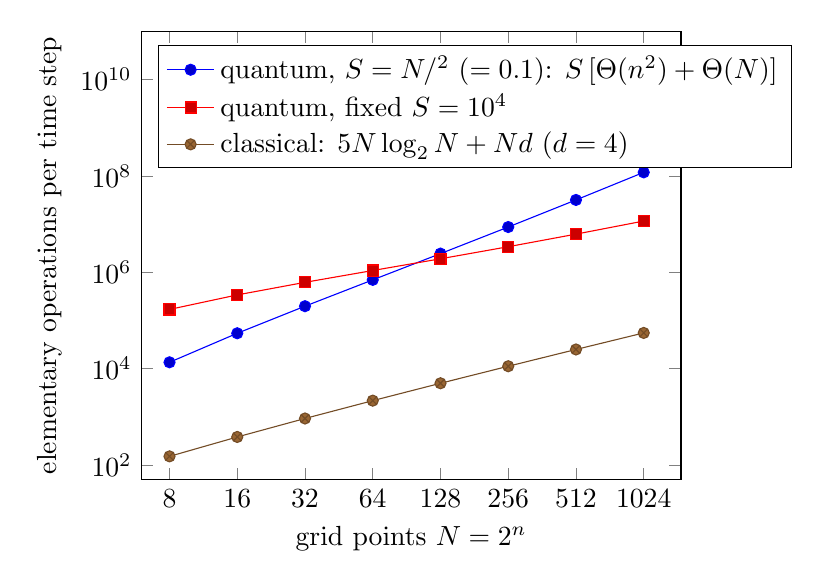
\begin{tikzpicture}
\begin{loglogaxis}[
  xlabel={grid points $N=2^{n}$},
  ylabel={elementary operations per time step},
  xmin=6,xmax=1500,ymin=50,ymax=1e11,
  xtick={8,16,32,64,128,256,512,1024},
  xticklabels={8,16,32,64,128,256,512,1024},
  legend pos=north west,
  legend cell align=left]
\addplot coordinates {(8,13600) (16,54400) (32,198400) (64,697600) (128,2444800) (256,8704000) (512,31744000) (1024,118681600)};
\addlegendentry{quantum, $S=N/\eps^{2}$ ($\eps=0.1$): $S\,[\Theta(n^{2})+\Theta(N)]$}
\addplot coordinates {(8,170000) (16,340000) (32,620000) (64,1090000) (128,1910000) (256,3400000) (512,6200000) (1024,11590000)};
\addlegendentry{quantum, fixed $S=10^{4}$}
\addplot coordinates {(8,152) (16,384) (32,928) (64,2176) (128,4992) (256,11264) (512,25088) (1024,55296)};
\addlegendentry{classical: $5N\log_2 N + Nd$ ($d=4$)}
\end{loglogaxis}
\end{tikzpicture}
\caption{Per-step cost of the hybrid quantum solver against the classical split-step solver as a function of grid size, evaluated from the cost model of \cref{eq:syn:costq,eq:syn:costc} with gate executions and floating-point operations placed on a common axis. Illustrative rendering of the model in \cite{guo2026nonlinearwaves}, not measured data; the slopes, not the absolute offsets, carry the conclusion.}
\label{fig:syn:cost}
\end{figure}

\subsection{What the Negative Result Means}\label{sec:syn:waves-meaning}

The direct route fails for a reason that has nothing to do with today's noise and everything to do with information: a nonlinear update needs $N$ numbers that a quantum register does not release for less than $\Theta(N)$ shots. Any proposal for end-to-end quantum advantage in nonlinear wave simulation must therefore contain a \emph{coherent} nonlinear update whose cost per step is $o(N)$ in gates and shots combined, and the model of \cref{sec:syn:costmodel} gives the target concretely: match the $\Theta(n^{2})$ cost of the linear kernel, or at least beat $\Theta(N\log N)$ with a constant that survives the shot overhead of reading the final answer. The linear-embedding routes can in principle meet this target for weakly nonlinear, dissipative problems~\cite{liu2021carleman}, and the polynomial arithmetic on encoded states developed in \cref{ch:qml} (\nnqa{}) is a candidate primitive for the pointwise polynomial map in \cref{eq:syn:poly} without measurement; the study of this chapter tells us how good such a primitive has to be. It also gives a template for honest accounting that applies beyond fluids: whenever an algorithm's inner loop needs the data it is processing, count the read-out.

\section{Relation to the Other Chapters}\label{sec:syn:relation}

Both halves of this chapter rest on the HPC stack of \cref{ch:qgear}. \rubriq{} places \cudaq{} state-vector simulation inside a reinforcement-learning loop on Perlmutter, using the same containers, Slurm integration and \qiskit{}-to-\cudaq{} lowering that \qgear{} provides; the nonlinear-wave study used GPU simulation to run the end-to-end hybrid solver at sizes beyond what the hardware runs covered. The data-encoding family in the \rubriq{} benchmark and the reload step of the split-step solver are both \qcrank{}-type vectorized encoders, so the encoding work of \cref{ch:qml} supplies the loader whose $\Theta(N)$ cost \cref{eq:syn:costq} counts, and \nnqa{} from the same chapter is the natural candidate for a coherent nonlinear update. The T-count that \rubriq{} minimizes is the fault-tolerant cost defined by the error-correcting codes of \cref{ch:qec}, and its Clifford-fraction term is a tableau check in the stabilizer formalism that \cref{ch:qec} uses to build and audit encoders; in the other direction, the seeded Clifford ensembles of \cref{ch:qec} are exactly the class of circuits that the Clifford term can verify at zero simulation cost. Finally, the cost discipline of Part~B---count shots, count depth, count reload latency, and compare with the classical baseline at equal accuracy---is the same discipline that the hardware-aware optimizers of \cref{ch:nisq} applied to NISQ circuits, carried into the fault-tolerant setting.

\section{Summary}\label{sec:syn:summary}

This chapter answered RQ4 in two parts. Learned synthesis can produce circuits that respect fault-tolerant budgets when the learning signal is a dense, decomposable rubric evaluated at HPC scale: \rubriq{} fine-tunes a 7B coder with GRPO against a five-term rubric computed by \cudaq{} simulation on Perlmutter and, on \num{1500} benchmark circuits, achieves $3.31\times$ mean T-gate compression against $2.05\times$ for sparse-reward RL, sub-$1\%$ hardware-constraint violations, $96\%$ correctness and two-to-three-fold faster convergence with proportionally fewer simulator calls, with circuits validated on IBM Heron~r3 and IonQ Forte~\cite{guo2026rubriq}. Honest cost accounting, applied to the direct simulation of nonlinear waves, shows that reading the field at every step costs $\Theta(N^{2}/\eps^{2})$ gate executions per step against $\Theta(N\log N)$ classically, so that no end-to-end advantage is possible without a coherent nonlinear update, and the unified cost-and-error model together with its adaptive controller and hardware-validated kernels states that target quantitatively~\cite{guo2026nonlinearwaves}. The next chapter turns from what fault-tolerant computation costs to whether it can be trusted when it runs on hardware the user does not own.
